% Created by tikzDevice version 0.12 on 2018-08-21 16:29:42
% !TEX encoding = UTF-8 Unicode
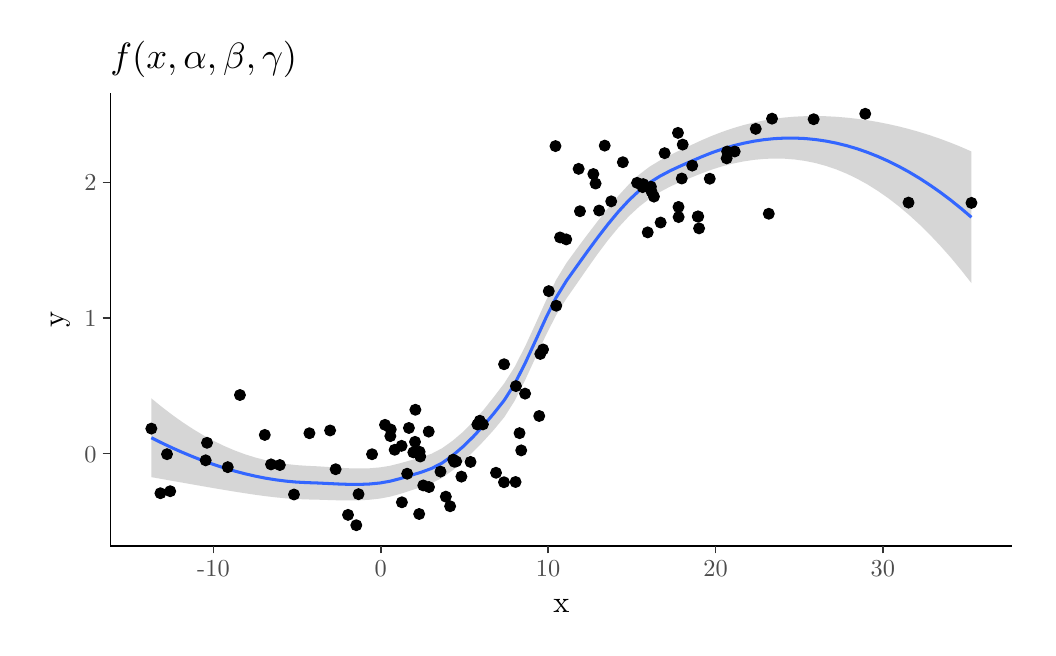
\begin{tikzpicture}[x=1pt,y=1pt]
\definecolor{fillColor}{RGB}{255,255,255}
\path[use as bounding box,fill=fillColor,fill opacity=0.00] (0,0) rectangle (361.35,216.81);
\begin{scope}
\path[clip] (  0.00,  0.00) rectangle (361.35,216.81);
\definecolor{drawColor}{RGB}{255,255,255}
\definecolor{fillColor}{RGB}{255,255,255}

\path[draw=drawColor,line width= 0.6pt,line join=round,line cap=round,fill=fillColor] (  0.00,  0.00) rectangle (361.35,216.81);
\end{scope}
\begin{scope}
\path[clip] ( 29.87, 29.59) rectangle (355.85,193.12);
\definecolor{fillColor}{RGB}{255,255,255}

\path[fill=fillColor] ( 29.87, 29.59) rectangle (355.85,193.12);
\definecolor{fillColor}{RGB}{153,153,153}

\path[fill=fillColor,fill opacity=0.40] ( 44.69, 82.86) --
	( 48.44, 79.80) --
	( 52.19, 76.93) --
	( 55.94, 74.26) --
	( 59.69, 71.80) --
	( 63.44, 69.54) --
	( 67.19, 67.50) --
	( 70.94, 65.68) --
	( 74.70, 64.07) --
	( 78.45, 62.68) --
	( 82.20, 61.50) --
	( 85.95, 60.53) --
	( 89.70, 59.75) --
	( 93.45, 59.15) --
	( 97.20, 58.73) --
	(100.95, 58.48) --
	(104.71, 58.31) --
	(108.46, 58.07) --
	(112.21, 57.82) --
	(115.96, 57.61) --
	(119.71, 57.52) --
	(123.46, 57.59) --
	(127.21, 57.90) --
	(130.96, 58.50) --
	(134.72, 59.44) --
	(138.47, 60.51) --
	(142.22, 61.52) --
	(145.97, 62.86) --
	(149.72, 64.82) --
	(153.47, 67.48) --
	(157.22, 70.66) --
	(160.97, 74.40) --
	(164.73, 78.69) --
	(168.48, 83.41) --
	(172.23, 88.33) --
	(175.98, 94.24) --
	(179.73,101.57) --
	(183.48,109.73) --
	(187.23,118.04) --
	(190.98,125.70) --
	(194.74,131.86) --
	(198.49,137.00) --
	(202.24,142.02) --
	(205.99,146.91) --
	(209.74,151.63) --
	(213.49,156.10) --
	(217.24,160.19) --
	(220.99,163.74) --
	(224.74,166.58) --
	(228.50,168.86) --
	(232.25,170.83) --
	(236.00,172.64) --
	(239.75,174.38) --
	(243.50,176.11) --
	(247.25,177.72) --
	(251.00,179.17) --
	(254.75,180.45) --
	(258.51,181.56) --
	(262.26,182.50) --
	(266.01,183.27) --
	(269.76,183.89) --
	(273.51,184.34) --
	(277.26,184.66) --
	(281.01,184.83) --
	(284.76,184.87) --
	(288.52,184.80) --
	(292.27,184.60) --
	(296.02,184.29) --
	(299.77,183.87) --
	(303.52,183.34) --
	(307.27,182.71) --
	(311.02,181.96) --
	(314.77,181.12) --
	(318.53,180.16) --
	(322.28,179.09) --
	(326.03,177.92) --
	(329.78,176.63) --
	(333.53,175.23) --
	(337.28,173.71) --
	(341.03,172.07) --
	(341.03,124.50) --
	(337.28,129.26) --
	(333.53,133.77) --
	(329.78,138.00) --
	(326.03,141.97) --
	(322.28,145.67) --
	(318.53,149.10) --
	(314.77,152.27) --
	(311.02,155.16) --
	(307.27,157.78) --
	(303.52,160.13) --
	(299.77,162.21) --
	(296.02,164.02) --
	(292.27,165.56) --
	(288.52,166.84) --
	(284.76,167.87) --
	(281.01,168.64) --
	(277.26,169.17) --
	(273.51,169.46) --
	(269.76,169.53) --
	(266.01,169.38) --
	(262.26,169.02) --
	(258.51,168.45) --
	(254.75,167.68) --
	(251.00,166.71) --
	(247.25,165.54) --
	(243.50,164.17) --
	(239.75,162.65) --
	(236.00,161.13) --
	(232.25,159.44) --
	(228.50,157.45) --
	(224.74,155.05) --
	(220.99,152.15) --
	(217.24,148.67) --
	(213.49,144.63) --
	(209.74,140.08) --
	(205.99,135.10) --
	(202.24,129.81) --
	(198.49,124.39) --
	(194.74,119.02) --
	(190.98,112.97) --
	(187.23,105.62) --
	(183.48, 97.55) --
	(179.73, 89.41) --
	(175.98, 81.98) --
	(172.23, 76.08) --
	(168.48, 71.53) --
	(164.73, 67.39) --
	(160.97, 63.56) --
	(157.22, 59.99) --
	(153.47, 56.78) --
	(149.72, 54.12) --
	(145.97, 52.22) --
	(142.22, 50.81) --
	(138.47, 49.59) --
	(134.72, 48.37) --
	(130.96, 47.34) --
	(127.21, 46.64) --
	(123.46, 46.22) --
	(119.71, 46.01) --
	(115.96, 45.96) --
	(112.21, 46.02) --
	(108.46, 46.13) --
	(104.71, 46.25) --
	(100.95, 46.33) --
	( 97.20, 46.47) --
	( 93.45, 46.73) --
	( 89.70, 47.08) --
	( 85.95, 47.52) --
	( 82.20, 48.03) --
	( 78.45, 48.59) --
	( 74.70, 49.18) --
	( 70.94, 49.80) --
	( 67.19, 50.43) --
	( 63.44, 51.08) --
	( 59.69, 51.74) --
	( 55.94, 52.40) --
	( 52.19, 53.06) --
	( 48.44, 53.73) --
	( 44.69, 54.39) --
	cycle;
\definecolor{drawColor}{RGB}{51,102,255}

\path[draw=drawColor,line width= 1.1pt,line join=round] ( 44.69, 68.63) --
	( 48.44, 66.76) --
	( 52.19, 64.99) --
	( 55.94, 63.33) --
	( 59.69, 61.77) --
	( 63.44, 60.31) --
	( 67.19, 58.97) --
	( 70.94, 57.74) --
	( 74.70, 56.62) --
	( 78.45, 55.63) --
	( 82.20, 54.77) --
	( 85.95, 54.02) --
	( 89.70, 53.42) --
	( 93.45, 52.94) --
	( 97.20, 52.60) --
	(100.95, 52.41) --
	(104.71, 52.28) --
	(108.46, 52.10) --
	(112.21, 51.92) --
	(115.96, 51.79) --
	(119.71, 51.76) --
	(123.46, 51.91) --
	(127.21, 52.27) --
	(130.96, 52.92) --
	(134.72, 53.90) --
	(138.47, 55.05) --
	(142.22, 56.17) --
	(145.97, 57.54) --
	(149.72, 59.47) --
	(153.47, 62.13) --
	(157.22, 65.33) --
	(160.97, 68.98) --
	(164.73, 73.04) --
	(168.48, 77.47) --
	(172.23, 82.21) --
	(175.98, 88.11) --
	(179.73, 95.49) --
	(183.48,103.64) --
	(187.23,111.83) --
	(190.98,119.33) --
	(194.74,125.44) --
	(198.49,130.69) --
	(202.24,135.91) --
	(205.99,141.00) --
	(209.74,145.85) --
	(213.49,150.36) --
	(217.24,154.43) --
	(220.99,157.95) --
	(224.74,160.82) --
	(228.50,163.16) --
	(232.25,165.14) --
	(236.00,166.88) --
	(239.75,168.52) --
	(243.50,170.14) --
	(247.25,171.63) --
	(251.00,172.94) --
	(254.75,174.07) --
	(258.51,175.00) --
	(262.26,175.76) --
	(266.01,176.33) --
	(269.76,176.71) --
	(273.51,176.90) --
	(277.26,176.91) --
	(281.01,176.74) --
	(284.76,176.37) --
	(288.52,175.82) --
	(292.27,175.08) --
	(296.02,174.15) --
	(299.77,173.04) --
	(303.52,171.73) --
	(307.27,170.24) --
	(311.02,168.56) --
	(314.77,166.69) --
	(318.53,164.63) --
	(322.28,162.38) --
	(326.03,159.94) --
	(329.78,157.32) --
	(333.53,154.50) --
	(337.28,151.49) --
	(341.03,148.29);
\definecolor{drawColor}{RGB}{0,0,0}
\definecolor{fillColor}{RGB}{0,0,0}

\path[draw=drawColor,line width= 0.4pt,line join=round,line cap=round,fill=fillColor] (188.30,121.61) circle (  1.96);

\path[draw=drawColor,line width= 0.4pt,line join=round,line cap=round,fill=fillColor] (236.35,162.30) circle (  1.96);

\path[draw=drawColor,line width= 0.4pt,line join=round,line cap=round,fill=fillColor] (242.11,148.56) circle (  1.96);

\path[draw=drawColor,line width= 0.4pt,line join=round,line cap=round,fill=fillColor] (115.76, 40.76) circle (  1.96);

\path[draw=drawColor,line width= 0.4pt,line join=round,line cap=round,fill=fillColor] (111.29, 57.25) circle (  1.96);

\path[draw=drawColor,line width= 0.4pt,line join=round,line cap=round,fill=fillColor] (199.09,165.79) circle (  1.96);

\path[draw=drawColor,line width= 0.4pt,line join=round,line cap=round,fill=fillColor] (109.28, 71.26) circle (  1.96);

\path[draw=drawColor,line width= 0.4pt,line join=round,line cap=round,fill=fillColor] (176.30, 52.64) circle (  1.96);

\path[draw=drawColor,line width= 0.4pt,line join=round,line cap=round,fill=fillColor] (263.09,180.24) circle (  1.96);

\path[draw=drawColor,line width= 0.4pt,line join=round,line cap=round,fill=fillColor] (240.14,166.97) circle (  1.96);

\path[draw=drawColor,line width= 0.4pt,line join=round,line cap=round,fill=fillColor] (220.21,160.74) circle (  1.96);

\path[draw=drawColor,line width= 0.4pt,line join=round,line cap=round,fill=fillColor] (137.76, 72.16) circle (  1.96);

\path[draw=drawColor,line width= 0.4pt,line join=round,line cap=round,fill=fillColor] ( 91.11, 58.77) circle (  1.96);

\path[draw=drawColor,line width= 0.4pt,line join=round,line cap=round,fill=fillColor] (252.76,172.06) circle (  1.96);

\path[draw=drawColor,line width= 0.4pt,line join=round,line cap=round,fill=fillColor] (129.12, 73.29) circle (  1.96);

\path[draw=drawColor,line width= 0.4pt,line join=round,line cap=round,fill=fillColor] ( 96.23, 48.12) circle (  1.96);

\path[draw=drawColor,line width= 0.4pt,line join=round,line cap=round,fill=fillColor] (137.13, 55.63) circle (  1.96);

\path[draw=drawColor,line width= 0.4pt,line join=round,line cap=round,fill=fillColor] (149.17, 56.40) circle (  1.96);

\path[draw=drawColor,line width= 0.4pt,line join=round,line cap=round,fill=fillColor] (140.10, 78.74) circle (  1.96);

\path[draw=drawColor,line width= 0.4pt,line join=round,line cap=round,fill=fillColor] ( 64.81, 66.80) circle (  1.96);

\path[draw=drawColor,line width= 0.4pt,line join=round,line cap=round,fill=fillColor] (236.69,174.56) circle (  1.96);

\path[draw=drawColor,line width= 0.4pt,line join=round,line cap=round,fill=fillColor] ( 44.69, 71.93) circle (  1.96);

\path[draw=drawColor,line width= 0.4pt,line join=round,line cap=round,fill=fillColor] (225.20,159.34) circle (  1.96);

\path[draw=drawColor,line width= 0.4pt,line join=round,line cap=round,fill=fillColor] (101.81, 70.26) circle (  1.96);

\path[draw=drawColor,line width= 0.4pt,line join=round,line cap=round,fill=fillColor] (153.77, 60.72) circle (  1.96);

\path[draw=drawColor,line width= 0.4pt,line join=round,line cap=round,fill=fillColor] (255.48,172.06) circle (  1.96);

\path[draw=drawColor,line width= 0.4pt,line join=round,line cap=round,fill=fillColor] ( 72.30, 58.00) circle (  1.96);

\path[draw=drawColor,line width= 0.4pt,line join=round,line cap=round,fill=fillColor] (162.51, 73.41) circle (  1.96);

\path[draw=drawColor,line width= 0.4pt,line join=round,line cap=round,fill=fillColor] (206.49,150.73) circle (  1.96);

\path[draw=drawColor,line width= 0.4pt,line join=round,line cap=round,fill=fillColor] (151.10, 47.34) circle (  1.96);

\path[draw=drawColor,line width= 0.4pt,line join=round,line cap=round,fill=fillColor] (163.37, 74.78) circle (  1.96);

\path[draw=drawColor,line width= 0.4pt,line join=round,line cap=round,fill=fillColor] (177.73, 70.29) circle (  1.96);

\path[draw=drawColor,line width= 0.4pt,line join=round,line cap=round,fill=fillColor] (228.72,146.39) circle (  1.96);

\path[draw=drawColor,line width= 0.4pt,line join=round,line cap=round,fill=fillColor] ( 47.97, 48.58) circle (  1.96);

\path[draw=drawColor,line width= 0.4pt,line join=round,line cap=round,fill=fillColor] (192.37,141.01) circle (  1.96);

\path[draw=drawColor,line width= 0.4pt,line join=round,line cap=round,fill=fillColor] (242.32,148.59) circle (  1.96);

\path[draw=drawColor,line width= 0.4pt,line join=round,line cap=round,fill=fillColor] (191.01,116.33) circle (  1.96);

\path[draw=drawColor,line width= 0.4pt,line join=round,line cap=round,fill=fillColor] (222.44,160.27) circle (  1.96);

\path[draw=drawColor,line width= 0.4pt,line join=round,line cap=round,fill=fillColor] (141.47, 41.08) circle (  1.96);

\path[draw=drawColor,line width= 0.4pt,line join=round,line cap=round,fill=fillColor] ( 85.68, 69.65) circle (  1.96);

\path[draw=drawColor,line width= 0.4pt,line join=round,line cap=round,fill=fillColor] (139.35, 63.35) circle (  1.96);

\path[draw=drawColor,line width= 0.4pt,line join=round,line cap=round,fill=fillColor] (267.80,149.57) circle (  1.96);

\path[draw=drawColor,line width= 0.4pt,line join=round,line cap=round,fill=fillColor] (318.29,153.60) circle (  1.96);

\path[draw=drawColor,line width= 0.4pt,line join=round,line cap=round,fill=fillColor] (252.58,169.59) circle (  1.96);

\path[draw=drawColor,line width= 0.4pt,line join=round,line cap=round,fill=fillColor] (341.03,153.49) circle (  1.96);

\path[draw=drawColor,line width= 0.4pt,line join=round,line cap=round,fill=fillColor] (204.40,163.92) circle (  1.96);

\path[draw=drawColor,line width= 0.4pt,line join=round,line cap=round,fill=fillColor] (234.98,178.79) circle (  1.96);

\path[draw=drawColor,line width= 0.4pt,line join=round,line cap=round,fill=fillColor] (210.86,154.05) circle (  1.96);

\path[draw=drawColor,line width= 0.4pt,line join=round,line cap=round,fill=fillColor] ( 87.94, 59.00) circle (  1.96);

\path[draw=drawColor,line width= 0.4pt,line join=round,line cap=round,fill=fillColor] (145.02, 50.81) circle (  1.96);

\path[draw=drawColor,line width= 0.4pt,line join=round,line cap=round,fill=fillColor] (160.03, 59.89) circle (  1.96);

\path[draw=drawColor,line width= 0.4pt,line join=round,line cap=round,fill=fillColor] (144.91, 70.85) circle (  1.96);

\path[draw=drawColor,line width= 0.4pt,line join=round,line cap=round,fill=fillColor] (169.24, 55.97) circle (  1.96);

\path[draw=drawColor,line width= 0.4pt,line join=round,line cap=round,fill=fillColor] (176.43, 87.29) circle (  1.96);

\path[draw=drawColor,line width= 0.4pt,line join=round,line cap=round,fill=fillColor] ( 51.51, 49.31) circle (  1.96);

\path[draw=drawColor,line width= 0.4pt,line join=round,line cap=round,fill=fillColor] (235.22,148.37) circle (  1.96);

\path[draw=drawColor,line width= 0.4pt,line join=round,line cap=round,fill=fillColor] (185.23, 98.91) circle (  1.96);

\path[draw=drawColor,line width= 0.4pt,line join=round,line cap=round,fill=fillColor] (242.61,144.29) circle (  1.96);

\path[draw=drawColor,line width= 0.4pt,line join=round,line cap=round,fill=fillColor] (172.15, 95.19) circle (  1.96);

\path[draw=drawColor,line width= 0.4pt,line join=round,line cap=round,fill=fillColor] (154.19, 59.94) circle (  1.96);

\path[draw=drawColor,line width= 0.4pt,line join=round,line cap=round,fill=fillColor] (139.97, 67.14) circle (  1.96);

\path[draw=drawColor,line width= 0.4pt,line join=round,line cap=round,fill=fillColor] (179.74, 84.57) circle (  1.96);

\path[draw=drawColor,line width= 0.4pt,line join=round,line cap=round,fill=fillColor] (135.22, 45.30) circle (  1.96);

\path[draw=drawColor,line width= 0.4pt,line join=round,line cap=round,fill=fillColor] (141.62, 63.55) circle (  1.96);

\path[draw=drawColor,line width= 0.4pt,line join=round,line cap=round,fill=fillColor] (224.05,142.84) circle (  1.96);

\path[draw=drawColor,line width= 0.4pt,line join=round,line cap=round,fill=fillColor] (118.75, 37.02) circle (  1.96);

\path[draw=drawColor,line width= 0.4pt,line join=round,line cap=round,fill=fillColor] (302.65,185.69) circle (  1.96);

\path[draw=drawColor,line width= 0.4pt,line join=round,line cap=round,fill=fillColor] (131.05, 69.22) circle (  1.96);

\path[draw=drawColor,line width= 0.4pt,line join=round,line cap=round,fill=fillColor] (268.97,183.93) circle (  1.96);

\path[draw=drawColor,line width= 0.4pt,line join=round,line cap=round,fill=fillColor] (164.49, 73.46) circle (  1.96);

\path[draw=drawColor,line width= 0.4pt,line join=round,line cap=round,fill=fillColor] (246.47,162.23) circle (  1.96);

\path[draw=drawColor,line width= 0.4pt,line join=round,line cap=round,fill=fillColor] (205.21,160.48) circle (  1.96);

\path[draw=drawColor,line width= 0.4pt,line join=round,line cap=round,fill=fillColor] (152.65, 43.88) circle (  1.96);

\path[draw=drawColor,line width= 0.4pt,line join=round,line cap=round,fill=fillColor] (194.62,140.30) circle (  1.96);

\path[draw=drawColor,line width= 0.4pt,line join=round,line cap=round,fill=fillColor] (230.16,171.46) circle (  1.96);

\path[draw=drawColor,line width= 0.4pt,line join=round,line cap=round,fill=fillColor] (131.20, 71.60) circle (  1.96);

\path[draw=drawColor,line width= 0.4pt,line join=round,line cap=round,fill=fillColor] (284.01,183.72) circle (  1.96);

\path[draw=drawColor,line width= 0.4pt,line join=round,line cap=round,fill=fillColor] (172.11, 52.55) circle (  1.96);

\path[draw=drawColor,line width= 0.4pt,line join=round,line cap=round,fill=fillColor] (222.21,159.20) circle (  1.96);

\path[draw=drawColor,line width= 0.4pt,line join=round,line cap=round,fill=fillColor] (156.73, 54.58) circle (  1.96);

\path[draw=drawColor,line width= 0.4pt,line join=round,line cap=round,fill=fillColor] (215.06,168.19) circle (  1.96);

\path[draw=drawColor,line width= 0.4pt,line join=round,line cap=round,fill=fillColor] (190.72,174.02) circle (  1.96);

\path[draw=drawColor,line width= 0.4pt,line join=round,line cap=round,fill=fillColor] (208.51,174.19) circle (  1.96);

\path[draw=drawColor,line width= 0.4pt,line join=round,line cap=round,fill=fillColor] ( 50.35, 62.69) circle (  1.96);

\path[draw=drawColor,line width= 0.4pt,line join=round,line cap=round,fill=fillColor] (235.18,152.03) circle (  1.96);

\path[draw=drawColor,line width= 0.4pt,line join=round,line cap=round,fill=fillColor] (119.56, 48.24) circle (  1.96);

\path[draw=drawColor,line width= 0.4pt,line join=round,line cap=round,fill=fillColor] ( 64.32, 60.47) circle (  1.96);

\path[draw=drawColor,line width= 0.4pt,line join=round,line cap=round,fill=fillColor] (178.34, 64.06) circle (  1.96);

\path[draw=drawColor,line width= 0.4pt,line join=round,line cap=round,fill=fillColor] (141.86, 61.84) circle (  1.96);

\path[draw=drawColor,line width= 0.4pt,line join=round,line cap=round,fill=fillColor] (186.23,100.53) circle (  1.96);

\path[draw=drawColor,line width= 0.4pt,line join=round,line cap=round,fill=fillColor] ( 76.70, 84.07) circle (  1.96);

\path[draw=drawColor,line width= 0.4pt,line join=round,line cap=round,fill=fillColor] (132.61, 64.27) circle (  1.96);

\path[draw=drawColor,line width= 0.4pt,line join=round,line cap=round,fill=fillColor] (154.84, 60.08) circle (  1.96);

\path[draw=drawColor,line width= 0.4pt,line join=round,line cap=round,fill=fillColor] (199.56,150.48) circle (  1.96);

\path[draw=drawColor,line width= 0.4pt,line join=round,line cap=round,fill=fillColor] (142.94, 51.40) circle (  1.96);

\path[draw=drawColor,line width= 0.4pt,line join=round,line cap=round,fill=fillColor] (225.41,157.65) circle (  1.96);

\path[draw=drawColor,line width= 0.4pt,line join=round,line cap=round,fill=fillColor] (184.85, 76.49) circle (  1.96);

\path[draw=drawColor,line width= 0.4pt,line join=round,line cap=round,fill=fillColor] (226.30,155.76) circle (  1.96);

\path[draw=drawColor,line width= 0.4pt,line join=round,line cap=round,fill=fillColor] (135.11, 65.70) circle (  1.96);

\path[draw=drawColor,line width= 0.4pt,line join=round,line cap=round,fill=fillColor] (124.44, 62.67) circle (  1.96);
\end{scope}
\begin{scope}
\path[clip] (  0.00,  0.00) rectangle (361.35,216.81);
\definecolor{drawColor}{RGB}{0,0,0}

\path[draw=drawColor,line width= 0.6pt,line join=round] ( 29.87, 29.59) --
	( 29.87,193.12);
\end{scope}
\begin{scope}
\path[clip] (  0.00,  0.00) rectangle (361.35,216.81);
\definecolor{drawColor}{gray}{0.30}

\node[text=drawColor,anchor=base east,inner sep=0pt, outer sep=0pt, scale=  0.88] at ( 24.92, 59.86) {0};

\node[text=drawColor,anchor=base east,inner sep=0pt, outer sep=0pt, scale=  0.88] at ( 24.92,108.83) {1};

\node[text=drawColor,anchor=base east,inner sep=0pt, outer sep=0pt, scale=  0.88] at ( 24.92,157.81) {2};
\end{scope}
\begin{scope}
\path[clip] (  0.00,  0.00) rectangle (361.35,216.81);
\definecolor{drawColor}{gray}{0.20}

\path[draw=drawColor,line width= 0.6pt,line join=round] ( 27.12, 62.89) --
	( 29.87, 62.89);

\path[draw=drawColor,line width= 0.6pt,line join=round] ( 27.12,111.87) --
	( 29.87,111.87);

\path[draw=drawColor,line width= 0.6pt,line join=round] ( 27.12,160.84) --
	( 29.87,160.84);
\end{scope}
\begin{scope}
\path[clip] (  0.00,  0.00) rectangle (361.35,216.81);
\definecolor{drawColor}{RGB}{0,0,0}

\path[draw=drawColor,line width= 0.6pt,line join=round] ( 29.87, 29.59) --
	(355.85, 29.59);
\end{scope}
\begin{scope}
\path[clip] (  0.00,  0.00) rectangle (361.35,216.81);
\definecolor{drawColor}{gray}{0.20}

\path[draw=drawColor,line width= 0.6pt,line join=round] ( 67.13, 26.84) --
	( 67.13, 29.59);

\path[draw=drawColor,line width= 0.6pt,line join=round] (127.61, 26.84) --
	(127.61, 29.59);

\path[draw=drawColor,line width= 0.6pt,line join=round] (188.08, 26.84) --
	(188.08, 29.59);

\path[draw=drawColor,line width= 0.6pt,line join=round] (248.56, 26.84) --
	(248.56, 29.59);

\path[draw=drawColor,line width= 0.6pt,line join=round] (309.03, 26.84) --
	(309.03, 29.59);
\end{scope}
\begin{scope}
\path[clip] (  0.00,  0.00) rectangle (361.35,216.81);
\definecolor{drawColor}{gray}{0.30}

\node[text=drawColor,anchor=base,inner sep=0pt, outer sep=0pt, scale=  0.88] at ( 67.13, 18.58) {-10};

\node[text=drawColor,anchor=base,inner sep=0pt, outer sep=0pt, scale=  0.88] at (127.61, 18.58) {0};

\node[text=drawColor,anchor=base,inner sep=0pt, outer sep=0pt, scale=  0.88] at (188.08, 18.58) {10};

\node[text=drawColor,anchor=base,inner sep=0pt, outer sep=0pt, scale=  0.88] at (248.56, 18.58) {20};

\node[text=drawColor,anchor=base,inner sep=0pt, outer sep=0pt, scale=  0.88] at (309.03, 18.58) {30};
\end{scope}
\begin{scope}
\path[clip] (  0.00,  0.00) rectangle (361.35,216.81);
\definecolor{drawColor}{RGB}{0,0,0}

\node[text=drawColor,anchor=base,inner sep=0pt, outer sep=0pt, scale=  1.10] at (192.86,  5.50) {x};
\end{scope}
\begin{scope}
\path[clip] (  0.00,  0.00) rectangle (361.35,216.81);
\definecolor{drawColor}{RGB}{0,0,0}

\node[text=drawColor,rotate= 90.00,anchor=base,inner sep=0pt, outer sep=0pt, scale=  1.10] at ( 13.08,111.35) {y};
\end{scope}
\begin{scope}
\path[clip] (  0.00,  0.00) rectangle (361.35,216.81);
\definecolor{drawColor}{RGB}{0,0,0}

\node[text=drawColor,anchor=base west,inner sep=0pt, outer sep=0pt, scale=  1.32] at ( 29.87,202.22) {$f(x, \alpha, \beta, \gamma)$};
\end{scope}
\end{tikzpicture}
